\documentclass[10pt,a4paper]{report}
\usepackage[utf8]{inputenc}
\usepackage[russian]{babel}
\usepackage{amsmath}
\usepackage{amsfonts}
\usepackage{amssymb}
\usepackage{graphicx}
\usepackage{listings}

\usepackage[left=1.8cm, right=1cm, top=0.8cm, bottom=2cm, 
bindingoffset=0cm]{geometry}

\author{Кенть Никита}
\title{Лабораторная работа №6.\\
	SSL/TLC}
\begin{document}
	\maketitle
	\renewcommand{\thesection}{\arabic{section}}
	\tableofcontents
	\pagebreak
	
	\setcounter{totalnumber}{10}
	\setcounter{topnumber}{10}
	\setcounter{bottomnumber}{10}
	\renewcommand{\topfraction}{1}
	\renewcommand{\textfraction}{0}
	
	\section{Цель работы}
		Изучить лучшие практики по развертыванию SSL/TLS.
		Изучить основные уязвимости и атаки на SSL последнего времени - POODLE, 
		HeartBleed.
	\section{Изучение практик по развертыванию SSL/TLC}
		\begin{itemize}
			\item Качество защиты, обеспечиваемой TLS полностью зависит от секретного ключа, закладывающего основу безопасности, и сертификата, который сообщает о подлинности сервера для его посетителей.
			
			\item Необходимо защищать закрытые ключи, предоставляя доступ к ним как 
			можно меньшему числу сотрудников.
			
			\item Используйте 2048-битный RSA или 256-битные ECDSA закрытые ключи для всех ваших серверов. Ключи такой крепости безопасны и будут оставаться безопасными в течение значительного периода времени. Если у вас есть 1024-битные RSA ключи, то следует заменить их более сильными ключами как можно скорее.
			
			\item Защитите закрытый ключ
			
			\item Убедитесь, что ваши сертификаты охватывают все доменные имена, которые вы хотите использовать на сайте. 
			
			\item Приобретайте сертификаты у надежного удостоверяющего центра
			
			\item Использование безопасных алгоритмов шифрования (подойдут 
			симметричные алгоритмы с ключами более 128 бит).
			
			\item  Используйте надежные алгоритмы подписи сертификата

Безопасность сертификата зависит от длины закрытого ключа и прочности используемой функции хеширования. Сегодня большинство сертификатов используют алгоритм SHA1, который считается слабым.

			
			\item Отключение проверки безопасности по инициативе клиента.
		\end{itemize}
	\section{Уязвимости POODLE и HeartBleed}
		\begin{itemize}
			\item POODLE - тим атаки <<человек по середине>>.
			Атака POODLE (Padding Oracle On Downgraded Legacy Encryption) позволяет восстановить содержимое отдельных секретных идентификаторов, передаваемых внутри зашифрованного SSLv3-соединения, и по своей сути напоминает такие ранее известные виды атак на HTTPS, как BREACH, CRIME и BEAST, но значительно проще для эксплуатации и не требует выполнения каких-то особых условий. Проблеме подвержен любой сайт, допускающий установку защищённых соединений с использованием протокола SSLv3, даже если в качестве более приоритетного протокола указаны актуальные версии TLS. Для отката на SSLv3 атакующие могут воспользоваться особенностью современных браузеров переходить на более низкую версию протокола, в случае сбоя установки соединения. 
			
			\item Heartbleed (CVE-2014-0160) - ошибка (переполнение буфера) в 
			криптографическом программном обеспечении OpenSSL, позволяющая 
			несанкционированно читать память на сервере или на клиенте, в том числе 
			для извлечения закрытого ключа сервера. 
			Heartbleed осуществляется отправкой некорректно сформированного 
			Heartbeat-запроса, в котором реальный размер строки очень мал, а число, 
			символизирующее длину передаваемой строки, очень велико.
			Так можно получить в ответ от сервера больше всего скрытой информации.
			Таким образом, у жертвы возможно за один запрос узнать до 64 килобайт 
			памяти, которая была ранее использована OpenSSL.
		\end{itemize}
	
	\section{Изучение отчетов ресурса SSL Server Test}
		\subsection{Домен из раздела Recent Best}
			В качестве домена из раздела Recent Best был выбран домен eu-survey.zoho.com.
			Отчет представлен на рисунке~\ref{pics:survery}.
			
			\begin{figure}[h]
				\centering
				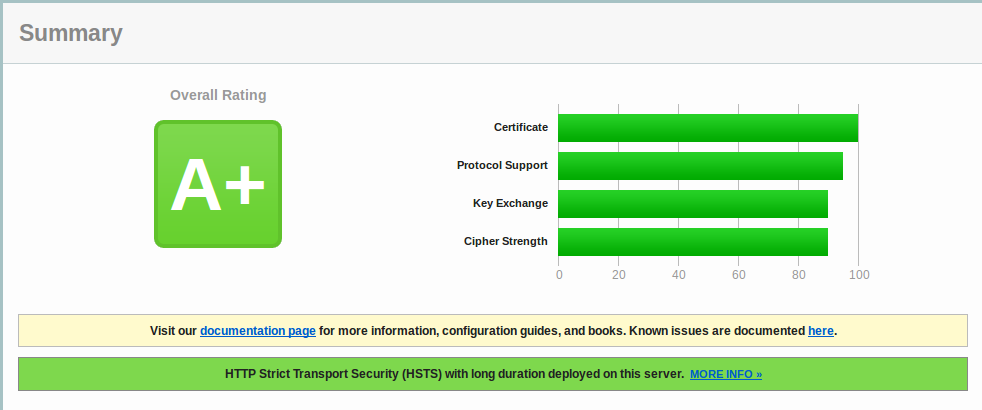
\includegraphics[width=0.9\textwidth]{pics/survery.png}
				\caption{Отчет для сайта eu-survey.zoho.com}
				\label{ris:survery}
			\end{figure}
			
			\begin{itemize}
				\item Поддерживает все типы протоколов TLS;
				\item Поддерживает форсированное защищённое соединение через протокол HTTPS.
			\end{itemize}
			
			В качестве домена из раздела Recent Worst был выбран домен 
			eu-static.zoho.com
			Отчет представлен на рисунке~\ref{ris:static}.
			
			\begin{figure}[h]
				\centering
				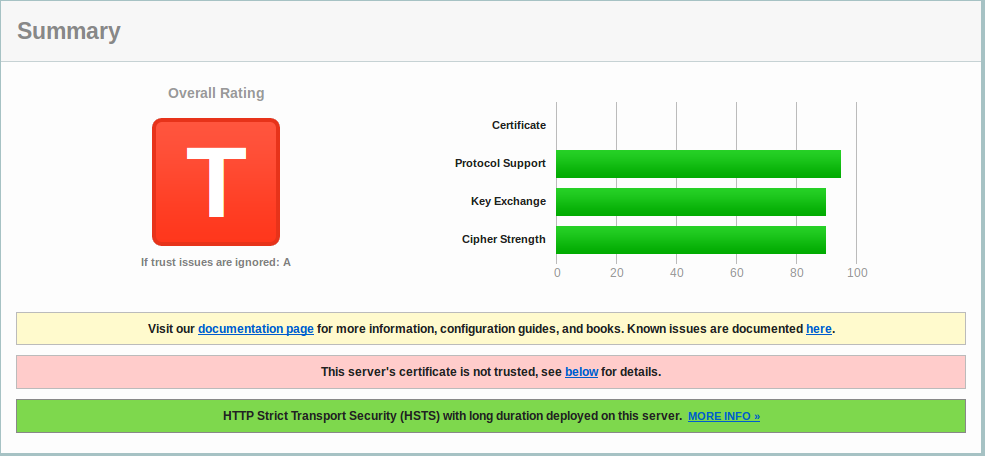
\includegraphics[width=0.9\textwidth]{pics/static.png}
				\caption{Отчет для сайта eu-static.zoho.com}
				\label{ris:static}
			\end{figure}
			
			\begin{itemize}
				\item Не доверенный сертификат
				\item Поддерживает форсированное защищённое соединение через протокол HTTPS.
			\end{itemize}
			
			Для самостоятельного анализа был выбран сервер github.com.
			Результаты анализа приведены на рисунке~\ref{ris:github}
			
			\begin{figure}[h]
				\centering
				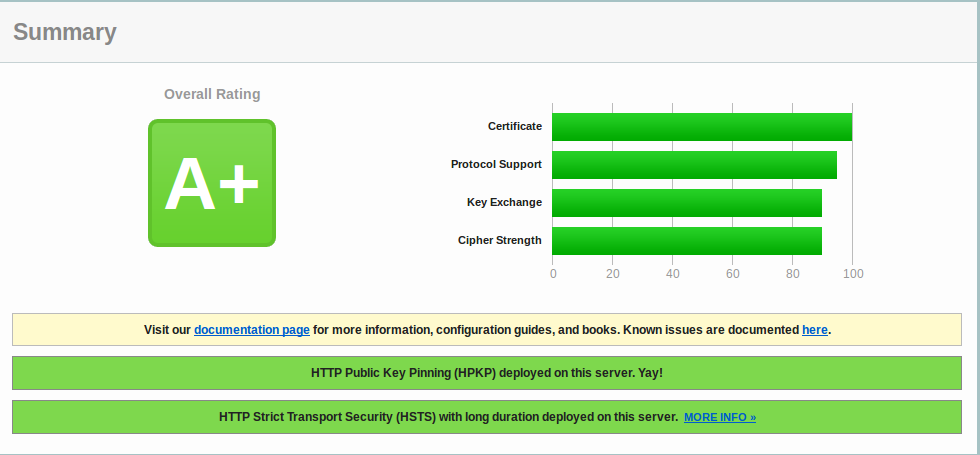
\includegraphics[width=0.9\textwidth]{pics/github.png}
				\caption{Отчет для сайта github.com}
				\label{ris:github}
			\end{figure}
			
			Как видно из рисунка~\ref{ris:github}, github.com поддерживает технологию HTTP Public Key Pinning, которая делает целевые атаки, связанные с Центрами Сертификации, намного более рискованными. Также поддерживает форсированное защищённое соединение через протокол
			
		\subsection{Расшифровка аббревиатур}
			Аббревиатуры представлены ниже:
			\begin{lstlisting}
TLS_ECDHE_RSA_WITH_AES_128_GCM_SHA256 (0xc02f)   ECDH secp256r1 (eq. 3072 bits RSA)   FS 	128
TLS_ECDHE_RSA_WITH_AES_256_GCM_SHA384 (0xc030)   ECDH secp256r1 (eq. 3072 bits RSA)   FS 	256
TLS_ECDHE_RSA_WITH_AES_128_CBC_SHA256 (0xc027)   ECDH secp256r1 (eq. 3072 bits RSA)   FS 	128
TLS_ECDHE_RSA_WITH_AES_128_CBC_SHA (0xc013)   ECDH secp256r1 (eq. 3072 bits RSA)   FS 	128
TLS_ECDHE_RSA_WITH_AES_256_CBC_SHA384 (0xc028)   ECDH secp256r1 (eq. 3072 bits RSA)   FS 	256
TLS_ECDHE_RSA_WITH_AES_256_CBC_SHA (0xc014)   ECDH secp256r1 (eq. 3072 bits RSA)   FS 	256
TLS_RSA_WITH_AES_128_GCM_SHA256 (0x9c) 	128
TLS_RSA_WITH_AES_256_GCM_SHA384 (0x9d) 	256
TLS_RSA_WITH_AES_128_CBC_SHA256 (0x3c) 	128
TLS_RSA_WITH_AES_128_CBC_SHA (0x2f) 	128
TLS_RSA_WITH_AES_256_CBC_SHA256 (0x3d) 	256
TLS_RSA_WITH_AES_256_CBC_SHA (0x35) 
			\end{lstlisting}
			
			Расшифровка аббревиатур:
			\begin{itemize}
				\item TLS\_ECDHE - алгоритм Диффи-Хэлмана на эллиптических кривых;
				\item RSA - алгоритм шифрования с открытым ключем;
				\item AES\_128 - алгоритм шифрования с длиной ключа в 128 бит;
				\item GCM и CBC - режимы блочного шифрования;
				\item SHA256 - хэш-функция с длиной ключа 256 бит.
			\end{itemize}
			
		\subsection{Protocol Details}
			Содержимое раздела Protocol Details представлено ниже:
			\begin{itemize}
				\item Проверка сертификата:
				\begin{lstlisting}
Secure Renegotiation	Supported
Secure Client-Initiated Renegotiation	No
Insecure Client-Initiated Renegotiation	No
				\end{lstlisting}
				
				\item Уязвимость к атакам Poodle, Bcast, Downgrade
				\begin{lstlisting}
BEAST attack: 	Not mitigated server-side (more info)   TLS 1.0: 0xc013
POODLE (SSLv3):	No, SSL 3 not supported (more info)
POODLE (TLS)	: 	No (more info)
Downgrade attack prevention	Yes, TLS_FALLBACK_SCSV supported (more info)
				\end{lstlisting}
				
				\item Слабый алгоритм RC4 не используется
				\begin{lstlisting}
RC4	No
				\end{lstlisting}
				
				\item Сервер защищен от атак HeartBleed
				\begin{lstlisting}
Heartbeat (extension)	Yes
Heartbleed (vulnerability)	No (more info)
				\end{lstlisting}
				
				\item Совместимость Forward Security с браузерами
				\begin{lstlisting}
Forward Secrecy	 	With modern browsers
				\end{lstlisting}
				
				\item Наличие NPN (отсутствует).

				\begin{lstlisting}
				NPN	 	No
				\end{lstlisting}
				
				\item Параметры сессии.
				\begin{lstlisting}
Session resumption (caching)	Yes
Session resumption (tickets)	No
				\end{lstlisting}
				
				\item Реализация HSTS.
				\begin{lstlisting}
Strict Transport Security (HSTS)	Yes
max-age=31536000;
HSTS Preloading	 	Chrome  Edge  Firefox  IE  Tor   
				\end{lstlisting}
				
				\item Реализация HPKP (отсутствует).
				\begin{lstlisting}
Public Key Pinning (HPKP)	Yes
				\end{lstlisting}
				
				\item Совместимость с SSL2 (совместим).
				\begin{lstlisting}
SSL 2 handshake compatibility	Yes
				\end{lstlisting}
			\end{itemize}
		
		\subsection{Вывод о реализации SSL на выбранном домене}
			Cервис github.com имеет хорошую конфигурацию: сервер 
			использует доверенный сертификат и защищен от основных типов атак.
			
			Cервис имеет поддержку Forward Security для большинства браузеров.
			Исходя из этого, можно сделать вывод о том, что сервис хорошо защищен.
	
	\section{Выводы}
		В данной работе мы изучили возможности, которые предоставляет сервис <<SSLLabs>>, 
		анализирующий качество защиты домена.
		Изучили отчеты, предоставляемые сервисом, а так же проанализировали 
		защиту сервиса github.com.
		Сервис позволяет увидеть защищенность домена от различных атак,
		список используемых протоколов, совместимость с различными браузерами и др.
\end{document}